% QSS manuscript variant — single-column journal format.
% Reuses the canonical section sources in ../paper/sections; the IEEE
% conference variant remains ../paper/main.tex. Numbers come from the
% same generated metrics macros (single source of numbers).
\documentclass[11pt,a4paper]{article}
\usepackage[utf8]{inputenc}
\usepackage[T1]{fontenc}
\usepackage{mathptmx}
\usepackage[margin=2.6cm]{geometry}
\usepackage{setspace}\onehalfspacing
\usepackage{graphicx}
\usepackage{booktabs}
\usepackage{tikz}
\usetikzlibrary{positioning,arrows.meta,shapes.geometric,fit}
\usepackage{xcolor}
\usepackage{url}
\usepackage[hidelinks]{hyperref}
\hypersetup{pdftitle={F(AI)2R: Who Did What, and Who Checked? Verifiable AI Provenance as an Executable Skill},
  pdfauthor={Florian Krebs}}
\graphicspath{{../paper/}}
% Generated by scripts/build_metrics.py - DO NOT EDIT BY HAND.
% Every number the paper cites comes from these macros; rerun the
% script to refresh all of them coherently (skill v0.15 rule).
\newcommand{\MTriples}{2\,110}
\newcommand{\MActivities}{142}
\newcommand{\MClaims}{8}
\newcommand{\MSources}{47}
\newcommand{\MSrcChecked}{40}
\newcommand{\MSrcSelf}{5}
\newcommand{\MHumanRungs}{6}
\newcommand{\MCommits}{124}
\newcommand{\MBookCommits}{51}
\newcommand{\MTurns}{2\,771}
\newcommand{\MOutTok}{1\,982\,634}
\newcommand{\MInTok}{15\,613}
\newcommand{\MCacheReadM}{562.4}
\newcommand{\MCacheWriteM}{23.3}
\newcommand{\MCacheReadMint}{562}
\newcommand{\MCostUSD}{1128}
\newcommand{\MOverReqPct}{11.6\%}
\newcommand{\MOverOutPct}{10.9\%}
\newcommand{\MOverCostPct}{7.9\%}
\newcommand{\MDirMsgs}{102}
\newcommand{\MDirWords}{1\,536}
\newcommand{\MDirMedian}{7}
\newcommand{\MActiveH}{9.2}
\newcommand{\MSpanH}{74}
\newcommand{\MPassAuth}{51}
\newcommand{\MPassAudit}{86}
\newcommand{\MPassRepair}{3}
\newcommand{\MPassBuild}{2}
\newcommand{\MProseWordsK}{8\,500}
\newcommand{\MToolLinesK}{2\,400}


\title{F(AI)\textsuperscript{2}R: Who Did What, and Who Checked?\\
\large Verifiable AI Provenance as an Executable Skill}
\author{Florian Krebs\\
\normalsize Deutsches Zentrum f\"ur Luft- und Raumfahrt (DLR)\\
\normalsize ORCID: 0000-0001-6033-801X}
\date{}

\begin{document}
\maketitle

\begin{abstract}
\noindent
F(AI)\textsuperscript{2}R is FAIR research with AI in the loop,
twice: an AI-assisted \emph{authoring} pass and a machine-readable
\emph{audit} pass over every artefact. AI systems now draft, refactor,
and verify research artefacts, yet their
contributions are rarely recorded in a form a later human or machine can
audit. Building on the original F(AI)\textsuperscript{2}R
experiment, we generalize its provenance model beyond scholarly writing into
\emph{aiprov}, a PROV-O extension covering any AI-in-the-loop artefact,
and we package the method as an \emph{executable skill} that an AI agent
operates itself: setup asks the human operator for their ORCID iD,
resolves their identity from the public registry, and scaffolds continuous
integration that gates every push on graph conformance and publishes the
current build of this very paper. The paper is its own case study. Every
activity, claim, and source in its production is recorded in the
repository's provenance graph under two invariants: no parentless claim,
and verification rungs that only humans may grant.

\medskip
\noindent\textbf{Keywords:} AI provenance; PROV-O; research integrity;
verification; agent skills; FAIR; human oversight
\end{abstract}

\section{Introduction}\label{sec:intro}
% Principal structure (authoring pass fills prose):
%
% P1  Hook: AI agents now draft, refactor, and verify research artefacts;
%     the work is real but evaporates at commit boundaries — a commit
%     records WHAT changed, not WHO (human or model) did it, at what cost,
%     from which sources. Cite the disclosure debate
%     \cite{chatgpt-wrote-it2023, chatgpt-priorities2023}.
% P2  Problem: existing answers are either policy (disclosure statements,
%     authorship bans) or documentation artefacts written after the fact
%     (model cards \cite{modelcards2019}); neither is machine-checkable at
%     the granularity of a claim.
% P3  Prior steps — the idea was sharpened across earlier experiments:
%     Obscurity-Is-Dead \cite{obscurity-is-dead} established
%     transcript-as-artifact and per-claim verification labels while
%     studying AI-compressed reverse-engineering effort;
%     F(AI)\textsuperscript{2}R \cite{fair2r-repo} — FAIR \cite{fair2016}
%     with AI in the loop, twice: authoring pass + audit pass over a
%     PROV-O graph \cite{prov-o2013}, under the no-parentless-claim
%     invariant — proved it on one scholarly paper, bound to paper
%     writing. NOTE for prose: this is a fast paper standing on slow
%     work — the experiments, HMC-context discussions, and exchanges
%     with colleagues (see Acknowledgment) did the sharpening. AI as
%     force multiplier: several strands (this method, this paper, a
%     system-integration fork of shepard \cite{shepard-fork}) advance
%     in parallel under one operator — which is precisely why
%     per-activity accounting matters: parallelism without provenance
%     is how contributions and errors alike become untraceable.
% P4  This paper's contributions:
%     (C1) aiprov: a domain-agnostic generalization of the F(AI)2R
%          vocabulary (any artefact, full inference telemetry);
%     (C2) the method packaged as an EXECUTABLE SKILL that the AI agent
%          operates itself — setup, logging, verification, CI/CD;
%     (C3) a meta-experiment: this paper is produced under the method,
%          and its provenance graph is the evaluation object.
% P5  Roadmap sentence.

\section{Background and Related Work}\label{sec:background}
% Principal structure:
%
% 2.1 Provenance models — PROV-O \cite{prov-o2013} and its lineage (OPM
%     \cite{opm2010}); PAV for authoring/versioning \cite{pav2013}.
%     Position: aiprov extends, never forks (subclassing prov: terms).
% 2.2 Contributor attribution — CRediT \cite{credit2019,credit-niso2022}:
%     role taxonomies name WHO contributed WHAT KIND of work, but at
%     manuscript granularity and human-only. aiprov records per-activity,
%     per-claim, and admits AI + tool agents.
% 2.3 AI transparency artefacts — model cards \cite{modelcards2019},
%     datasheets \cite{datasheets2021}: document the MODEL or the DATA,
%     not the collaboration that produced a specific artefact.
% 2.4 Research packaging — RO-Crate \cite{rocrate2022}: complementary;
%     aiprov graphs can travel inside a crate.
% 2.5 The trust gap — hallucinated citations \cite{ai-hallucination2023}
%     preview the systemic problem treated in §\ref{sec:dilution}: the
%     ladder makes existence machine-checkable and support a judgement
%     with an explicit grantor.
% 2.6 Lineage and neighbors — direct ancestors: Obscurity-Is-Dead
%     \cite{obscurity-is-dead} (transcript-as-artifact; the labels
%     repo-vendored / lit-read / unverified-external that this ladder
%     canonicalizes) and F(AI)2R \cite{fair2r-repo} (two-pass model,
%     no-parentless-claim). Adjacent DLR work extends PROV-O with
%     uncertainty quantification for engineering traceability
%     \cite{uncertainty-prov2026}: complementary axes — aiprov records
%     who/how work happened, uncertainty-aware provenance records how
%     confident results are; a combined profile is future work (§8).
%     A third root is industrial semantic modeling: the author
%     co-authored the Asset Administration Shell Part 1 specification
%     \cite{aas-part1-v30rc02} (now IDTA-01001 \cite{aas-part1-idta})
%     — where partners exchange information across a value chain,
%     semantics must be formal and machine-readable or interoperability
%     fails. aiprov applies that same discipline to a new exchange
%     relationship: the one between humans, AI agents, and future
%     auditors of their joint work.
% 2.7 Metadata-community context — the Helmholtz Metadata Collaboration
%     (HMC) \cite{hmc-conference2025} pushes FAIR metadata practice
%     across research infrastructures; a provenance graph is metadata
%     ABOUT WORK, so aiprov can be read as extending that programme
%     from data description to collaboration description.

\section{The Dilution Crisis}\label{sec:dilution}
% Principal structure:
%
% 3.1 The flood — scientific output growing faster than the capacity to
%     review it \cite{publishing-strain2024}; paper mills industrialize
%     fabrication \cite{paper-mills2021}; LLMs collapse the marginal cost
%     of a plausible paper to near zero, and GPT-fabricated papers are
%     already indexed and ranked by scholarly search engines
%     \cite{gpt-fabricated2024}.
% 3.2 Why finding good sources is hard now — retrieval trusted proxies
%     (indexed, cited, fluent) that generation has learned to imitate;
%     fabricated and erroneous citations propagate through reference
%     lists \cite{fabricated-citations2023, ai-hallucination2023}; the
%     feedback loop: models trained on the polluted pool degrade further
%     (model collapse) \cite{model-collapse2024} — dilution compounds.
% 3.3 Originality under dilution — when text is cheap, the scarce good is
%     an ORIGINAL idea whose support is checkable. Originality is itself
%     a provenance property: an idea's novelty claim needs a recorded
%     search horizon (what was looked for, where, when — §\ref{sec:method}
%     logs the sweeps) and every supporting or refuting fact attached.
% 3.4 The aiprov answer — claims are first-class: each assertion carries
%     wasGeneratedBy/wasAttributedTo and a ladder state separating
%     "the reference exists" (machine-checkable, reference-resolved)
%     from "the content supports the claim" (ai-confirmed at most, when
%     machine-judged) from "a human checked" (human-only rungs);
%     aiprov:contradicts makes refutation explicit instead of silent —
%     a claim REFUTED by facts is recorded as such, not deleted.
%     Supply-side transparency: artefacts carry verifiable pedigree, so
%     filtering the pool can shift from fluency heuristics to metadata
%     that fabrication cannot cheaply forge (DOIs that resolve, hashes,
%     commits, registry-resolved identities).

\section{The aiprov Method}\label{sec:method}

\textbf{Model.} aiprov extends PROV-O with three agent classes
(\texttt{HumanAgent}, \texttt{AIAgent}, \texttt{ToolAgent}), four
activity classes (\texttt{AuthoringPass}, \texttt{AuditPass},
\texttt{Build}, \texttt{Repair}), and entity classes for artefacts,
claims, sources, transcripts, and prompts, where prompts are treated
as source code and bound to activities as plans
(Figure~\ref{fig:vocab}). Humans carry ORCID and affiliation; AI
agents carry model, version, provider, endpoint, context window, and
knowledge cutoff; tool agents cover deterministic actors such as CI
jobs. Treating prompts as plans deserves a word: a prompt is to an AI
activity what a script is to a batch job, the executable
specification of intent, so it is hashed and bound with
\texttt{prov:hadPlan} rather than paraphrased into a comment. An
auditor who wants to know \emph{why} an artefact came out as it did
reads the plan and the transcript; neither is recoverable after the
fact if not captured when the activity runs.

\textbf{Telemetry.} Activities carry session and request identifiers,
token counts by class (input, output, cache, reasoning), sampling
parameters, cost, energy, and the tools invoked. One rule governs all
of it: omit, don't estimate. Absent telemetry is recorded as absent;
invented precision is worse than a visible gap. Generated artefacts
receive sha256 content hashes at logging time, and prompt files
receive prompt hashes.

\textbf{Invariant I: no parentless claim.} Every \texttt{aiprov:Claim}
needs a generating activity, an attributed agent, and a verification
state. The conformance validator treats violations as hard failures
and is suitable as a pre-commit hook or CI gate.

\textbf{Invariant II: the verification ladder.} Rungs answer who
checked what (Figure~\ref{fig:ladder}, Table~\ref{tab:ladder}).
Promotions must strictly climb and are themselves logged as audit
activities, so every rung a claim or source holds has a recorded
grantor. Disagreement is first-class: an agent may \emph{refuse} a
promotion, which changes no state but is logged as an audit activity
carrying the refused rung, so ``checked and not convinced'' is
distinguishable from ``never checked''. Rungs 5--6 are human-only; an AI-granted promotion to them is
a validator hard failure. Two rungs deserve comment. Vendoring
(rung~4) is not a verification statement: an unread vendored copy
proves nothing beyond \texttt{reference-resolved}. Its role is
instrumental, the access gate that makes human verification feasible
and durable. Operationally, the agent must hand the human the
evidence: \texttt{promote} refuses the human-only rungs unless the
source is vendored (path and hash recorded) or carries a clear access
link, and prints the review material with every request; a human
confirmation against link-only material is flagged, since the audit
target remains mutable. At the top, \texttt{human-read} subsumes
\texttt{human-confirmed}: it asserts full-text familiarity \emph{and}
confirmation, because a name alone would mislead, as reading does not
entail checking. Both refinements were operator-contested
mid-experiment (Section~\ref{sec:meta}). The ladder itself has
provenance: it canonicalizes labels field-tested in
\emph{Obscurity-Is-Dead}~\cite{obscurity-is-dead} and hardened in
F(AI)\textsuperscript{2}R~\cite{fair2r-repo}, and legacy names remain
machine-readable aliases, so that ancestor graphs can consolidate
onto this ladder without rewriting history; the aliases are in place,
though the consolidation has not yet been exercised against the
ancestor repositories' graphs.

\textbf{Commit binding.} An activity can only bind a commit that
already exists, and a commit cannot contain the graph entry describing
itself. The working discipline that follows: commit the artefacts, log
the activity with that commit's hash, then commit the graph update
separately. The graph never claims a hash it could not have known; the
cost is one extra commit per logged round. What the two commits buy
is tamper evidence in both directions. The graph entry names a commit
whose tree contains the artefacts it describes, content-hashed; the
graph itself lives in later commits of the same history. Backdating a
record would require rewriting published git history, and quietly
swapping an artefact would break its recorded hash: either
falsification is possible, but neither is silent, and that asymmetry,
honest work is cheap and dishonest work is loud, is the design goal
throughout.

\textbf{The validator, exhaustively.} Conformance is seven concrete
checks, each a SPARQL query over the graph, and naming them makes the
invariants operational rather than aspirational. Three enforce
Invariant~I: no claim without a generating activity, no claim without
an attributed agent, no activity without an associated agent. Two
enforce Invariant~II: no human-only rung granted by an AI agent, and
no human-only rung without a recorded promotion activity naming a
human grantor, which closes the loophole of a rung edited directly
into the graph without an audit trail. Two enforce the access gate:
no source above \texttt{needs-research} without a resolvable DOI, URL,
or vendored copy, and a warning, rather than a failure, for
human-verified sources whose audit target is link-only and therefore
mutable. Six checks are hard failures with a nonzero exit code;
that exit code is the entire integration contract, which is why the
same command serves unchanged as a pre-commit hook, a CI gate, and an
auditor's first step.

\textbf{Auditability operations.} \texttt{report} aggregates tokens,
cost, and rung distributions; \texttt{extract} computes the backward
closure of everything that contributed to chosen entities;
\texttt{dashboard} renders the graph as a self-contained offline
ledger. Sources enter through open registries (Crossref, OpenAlex,
arXiv, DataCite): a search command sweeps them, and registration with
DOI verification promotes a source to \texttt{reference-resolved} only
if the registry actually resolves it.

\begin{figure}[t]
\centering
\resizebox{\columnwidth}{!}{%
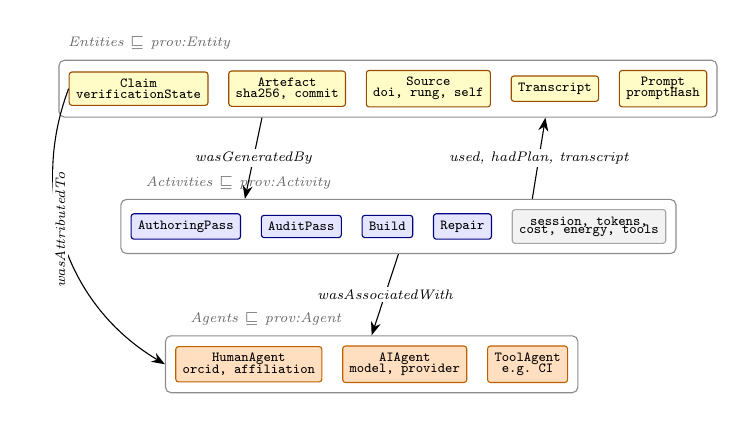
\begin{tikzpicture}[
  font=\scriptsize, node distance=2.5mm,
  ecls/.style={draw=orange!60!black, fill=yellow!22, rounded corners=1pt,
               inner sep=2.5pt, font=\tiny\ttfamily, align=center},
  acls/.style={draw=blue!50!black, fill=blue!10, rounded corners=1pt,
               inner sep=2.5pt, font=\tiny\ttfamily, align=center},
  gcls/.style={draw=orange!75!black, fill=orange!25, rounded corners=1pt,
               inner sep=2.5pt, font=\tiny\ttfamily, align=center},
  pkg/.style={draw=black!45, rounded corners=2pt, inner sep=3.5pt},
  pkl/.style={font=\tiny\itshape, text=black!60},
  e/.style={-{Stealth[length=1.7mm]}},
  lbl/.style={font=\tiny\itshape, fill=white, inner sep=1pt}]
% Entities (top)
\node[ecls] (claim) at (0,0)
  {Claim\\[-2pt]\tiny verificationState};
\node[ecls, right=of claim] (artefact)
  {Artefact\\[-2pt]\tiny sha256, commit};
\node[ecls, right=of artefact] (source)
  {Source\\[-2pt]\tiny doi, rung, self};
\node[ecls, right=of source] (transcript)
  {Transcript};
\node[ecls, right=of transcript] (prompt)
  {Prompt\\[-2pt]\tiny promptHash};
\node[pkg, fit=(claim)(prompt)] (epkg) {};
\node[pkl, anchor=south west] at (epkg.north west)
  {Entities \(\sqsubseteq\) prov:Entity};
% Activities (middle)
\node[acls] (auth) at (0.6,-1.75) {AuthoringPass};
\node[acls, right=of auth] (audit) {AuditPass};
\node[acls, right=of audit] (build) {Build};
\node[acls, right=of build] (repair) {Repair};
\node[acls, right=of repair, draw=black!35, fill=black!5]
  (tele) {\tiny session, tokens,\\[-3pt]\tiny cost, energy, tools};
\node[pkg, fit=(auth)(tele)] (apkg) {};
\node[pkl, anchor=south west] at ([xshift=2mm]apkg.north west)
  {Activities \(\sqsubseteq\) prov:Activity};
% Agents (bottom)
\node[gcls] (human) at (1.4,-3.5) {HumanAgent\\[-2pt]\tiny orcid, affiliation};
\node[gcls, right=of human] (ai) {AIAgent\\[-2pt]\tiny model, provider};
\node[gcls, right=of ai] (toolag) {ToolAgent\\[-2pt]\tiny e.g.\ CI};
\node[pkg, fit=(human)(toolag)] (gpkg) {};
\node[pkl, anchor=south west] at ([xshift=2mm]gpkg.north west)
  {Agents \(\sqsubseteq\) prov:Agent};
% properties
\draw[e] ([xshift=-16mm]epkg.south) -- ([xshift=-19.5mm]apkg.north)
  node[lbl, midway] {wasGeneratedBy};
\draw[e] ([xshift=17mm]apkg.north) -- ([xshift=20mm]epkg.south)
  node[lbl, midway] {used, hadPlan, transcript};
\draw[e] (apkg.south) -- (gpkg.north)
  node[lbl, midway] {wasAssociatedWith};
\draw[e] (claim.west) to[bend right=40]
  node[lbl, pos=0.45, rotate=90] {wasAttributedTo} (gpkg.west);
\end{tikzpicture}%
}
\caption{Core aiprov vocabulary as an extension of PROV-O. Every class
subclasses a \texttt{prov:} term; tiny annotations name characteristic
attributes. Claims point to their generating activity, their
attributed agent, and a verification state; activities carry inference
telemetry and link prompts (as plans) and transcripts.}
\label{fig:vocab}
\end{figure}

\begin{table*}[t]
\caption{The verification ladder. Positions are machine-readable
(\texttt{aiprov:ladderPosition}); promotions must strictly increase
them and are themselves logged as audit activities, so every rung a
claim or source holds has a recorded grantor.}
\label{tab:ladder}
\centering
\small
\begin{tabular}{clp{8.2cm}l}
\toprule
Pos & Rung & What it asserts & Who may grant \\
\midrule
0 & \texttt{unverified} & Recorded; nothing checked yet by anyone.
    Default state at creation. & (default) \\
1 & \texttt{needs-research} & A check was attempted or demanded and did
    \emph{not} succeed (e.g.\ a DOI failed to resolve). Must not be
    cited or relied upon until re-verified. & any agent \\
2 & \texttt{reference-resolved} & The reference \emph{exists}: its
    DOI/URL resolved in a bibliographic registry and metadata was
    captured. Says nothing about content. & any agent (tool-checkable) \\
3 & \texttt{ai-confirmed} & An AI checked that the source
    \emph{content} supports the associated claim. A machine judgement,
    the highest rung an AI may grant. & AI or human \\
4 & \texttt{source-vendored} & A copy of the source is preserved inside
    the repository (content-hashed), immune to link rot and silent
    revision. Of no evidential value by itself: this rung is the
    \emph{access gate} to human verification: the agent hands the
    human the evidence, and tooling refuses rungs 5--6 unless the
    source is vendored or carries a clear access link (DOI/URL). &
    any agent (hash-checkable) \\
5 & \texttt{human-confirmed} & A \emph{human} spot-checked that the
    source supports the claim. & human only \\
6 & \texttt{human-read} & A \emph{human} has read the source in full
    \emph{and}, with that full context, confirms the claim is
    supported, subsuming rung 5's confirmation with deeper
    familiarity. Reading without confirming is not a rung. Top of the
    ladder. & human only \\
\bottomrule
\end{tabular}
\end{table*}

\begin{figure}[t]
\centering
\resizebox{0.80\columnwidth}{!}{%
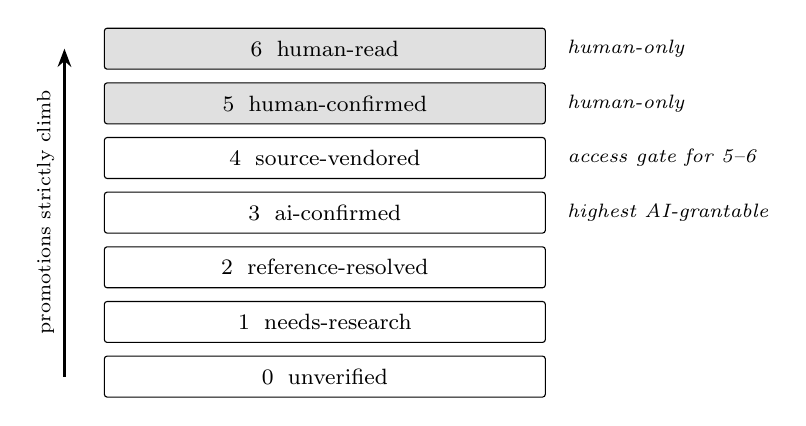
\begin{tikzpicture}[
  rung/.style={draw, rounded corners=1pt, minimum width=5.6cm,
               minimum height=0.52cm, font=\footnotesize, align=center},
  human/.style={rung, fill=black!12},
  note/.style={font=\scriptsize\itshape, anchor=west}]
\node[human] (r6) {6\; human-read};
\node[human, below=0.16cm of r6] (r5) {5\; human-confirmed};
\node[rung, below=0.16cm of r5] (r4) {4\; source-vendored};
\node[rung, below=0.16cm of r4] (r3) {3\; ai-confirmed};
\node[rung, below=0.16cm of r3] (r2) {2\; reference-resolved};
\node[rung, below=0.16cm of r2] (r1) {1\; needs-research};
\node[rung, below=0.16cm of r1] (r0) {0\; unverified};
\node[note, right=0.15cm of r6] {human-only};
\node[note, right=0.15cm of r5] {human-only};
\node[note, right=0.15cm of r4] {access gate for 5--6};
\node[note, right=0.15cm of r3] {highest AI-grantable};
\draw[-{Stealth}, thick] ([xshift=-0.5cm]r0.west) -- ([xshift=-0.5cm]r6.west)
  node[midway, sloped, above, font=\scriptsize] {promotions strictly climb};
\end{tikzpicture}%
}
\caption{The verification ladder. Every promotion is logged as an audit
activity; rungs 5--6 may never be granted by an AI agent, and the
validator treats such grants as hard failures.}
\label{fig:ladder}
\end{figure}

\section{The Executable Skill}\label{sec:skill}
% Principal structure:
%
% 4.1 From method description to executable procedure — a skill is a
%     versioned instruction+tool bundle the agent loads and OPERATES;
%     the method's rules become the agent's operating rules (log your own
%     activities; claims at most ai-confirmed; never fabricate telemetry).
% 4.2 ORCID-first setup — the only question asked of the human is their
%     ORCID iD; identity (name, affiliation) is resolved from the public
%     registry, not guessed; base IRI derives from the git remote; all
%     later commands auto-detect it. Figure~\ref{fig:workflow}.
% 4.3 CI/CD as the deterministic Build agent — every push: validate the
%     graph (invariants enforced server-side), render the dashboard,
%     compile the paper to PDF; the current paper version is always
%     available as a build artifact.
% 4.4 Versioning the method itself — the skill tree is the repository;
%     released snapshots are immutable (archive/), changes logged
%     (CHANGELOG), so the meta-experiment can cite the exact skill
%     version in force during each activity.
% 4.5 The skill as the transferable unit — the same skill that wrote
%     this paper is the integration payload for infrastructure
%     (shepard fork \cite{shepard-fork}, §8): packaging the method as
%     an operable bundle, not a PDF of guidelines, is what lets one
%     operator run several provenance-tracked strands in parallel —
%     the force-multiplier effect of §1 with its accounting built in.
% 4.6 Regulatory fit by construction — because the skill generates the
%     EU AI Act transparency statement from the graph (§ Ack.,
%     \cite{eu-ai-act2024}), disclosure is a build product, not an
%     authoring chore; adopters inherit it via init --paper.

\begin{figure}[t]
\centering
% TODO(F3): TikZ workflow loop: ORCID question -> init (seed graph,
% register human, scaffold CI) -> register AI agent -> work loop
% (log / claim / source --verify) -> validate -> push -> CI (validate,
% dashboard, PDF artifact) -> audit/promote (human rungs).
\fbox{\parbox[c][4.2cm][c]{0.9\linewidth}{\centering\itshape
F3 placeholder: skill workflow from ORCID question to CI artifact}}
\caption{The skill's operating loop from first setup question to
continuously published paper build.}
\label{fig:workflow}
\end{figure}

\section{Meta-Experiment: This Paper as Case Study}\label{sec:meta}
% Principal structure:
%
% 5.1 Setup — repository bootstrapped by the AI agent under the skill;
%     every commit paired with graph activities; agents: one human
%     (registry-resolved), one AI, CI as tool agent. The working
%     environment is Figure~\ref{fig:environment}: the operator's
%     conversation with the AI agent on the left, the continuously
%     rebuilt draft of this paper on the right — the loop of
%     §\ref{sec:skill}, in operation.

\begin{figure*}[t]
\centering
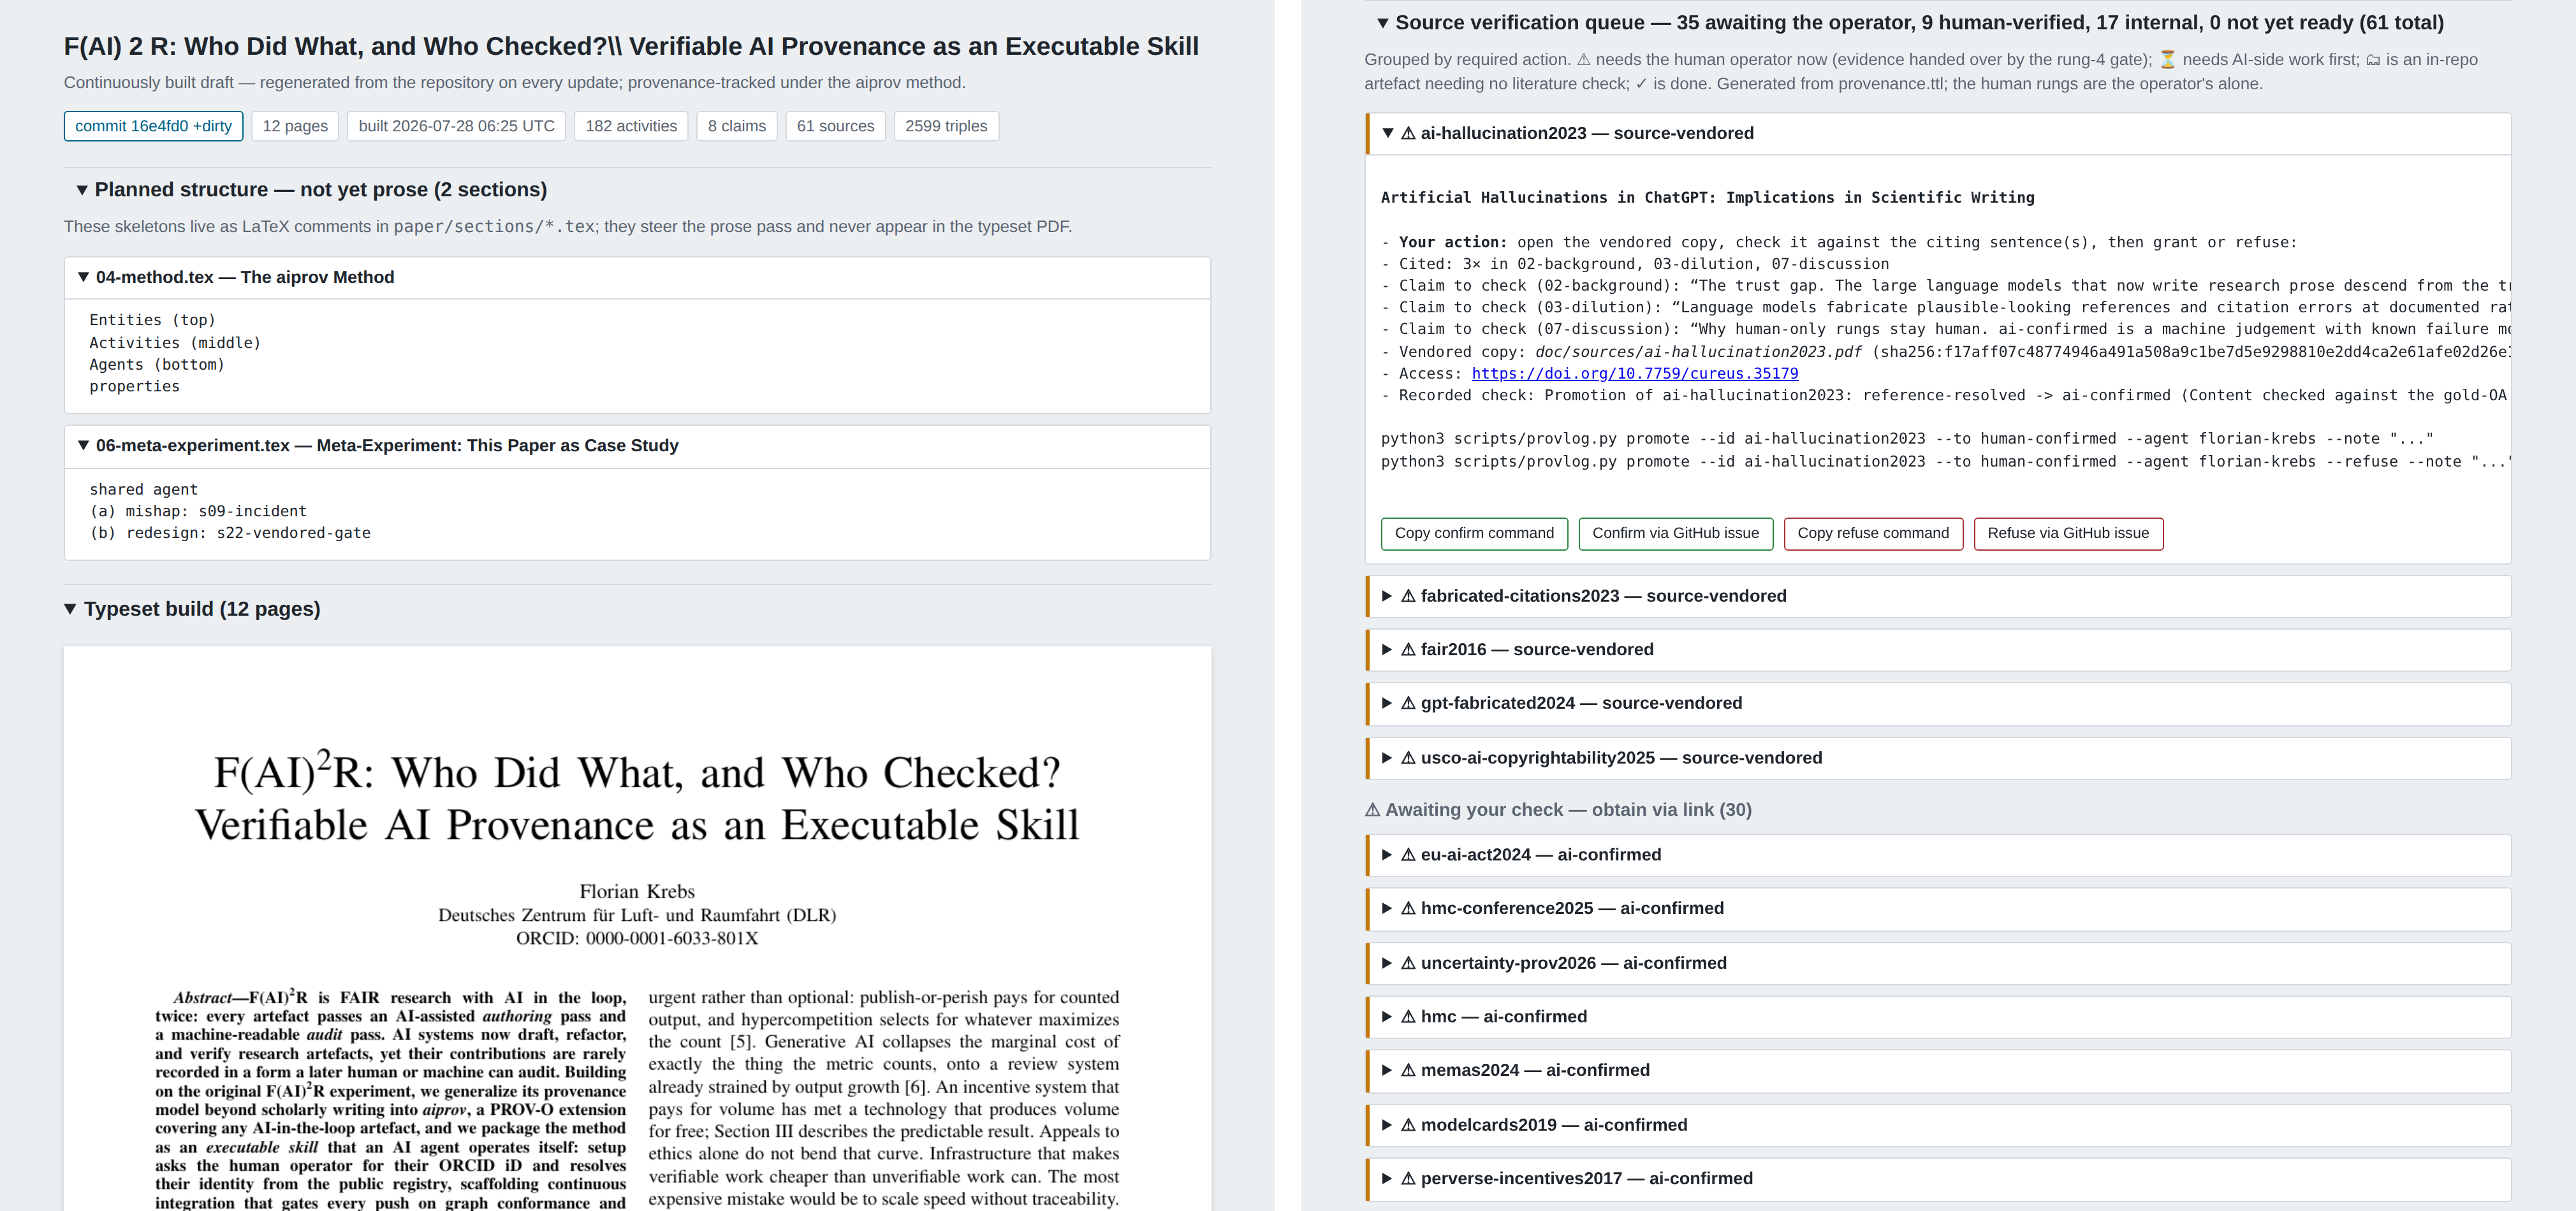
\includegraphics[width=\textwidth]{figures/environment.png}
\caption{The meta-experiment's working environment (screenshot,
2026-07-24): left, the session in which the human operator directs the
AI agent — visible are ORCID-resolved acknowledgement additions, a CI
check, and provenance-logged pushes; right, the continuously rebuilt
draft of this paper, republished to a stable preview URL after every
editing round, with commit, build time, and live provenance-graph
statistics in the header.}
\label{fig:environment}
\end{figure*}
% 5.2 The graph as evaluation object — counts of activities, claims,
%     sources by rung; Table~\ref{tab:telemetry}; Figure~\ref{fig:graph}
%     (extract of what contributed to this paper).
% 5.3 Worked examples — (a) invariant enforcement caught by test-run
%     before claims entered at ai-confirmed; (b) a source found via the
%     open-API sweep, DOI-verified, cited, then human-promoted; (c) the
%     ORCID-resolved agent registration logged as an audit activity;
%     (d) lineage as data: the paper's intellectual ancestors
%     (Obscurity-Is-Dead, F(AI)2R, uncertainty-aware provenance, AAS,
%     HMC, shepard) are registered graph sources, each fetched or
%     URL-verified before registration — including a recorded fallback
%     when a publisher blocked automated access (ResearchGate 403 ->
%     canonical Plattform Industrie 4.0 page); (e) a malformed
%     registry-supplied BibTeX entry broke the CI build, was diagnosed
%     from CI logs, fixed, and the first green run is itself a logged
%     Build activity by the CI ToolAgent with artifact digests.
% 5.3b Incidents as first-class records (Figure~\ref{fig:incident}) —
%     the experiment produced four incident types, and none needed a
%     special vocabulary; each is an ordinary activity whose class
%     carries its nature:
%     (i)   agent mishap — the section-overwrite (act s09-incident):
%           an AuditPass self-report naming what happened, the tools
%           involved, and the restoring commit; recovery was git,
%           the record is the graph;
%     (ii)  infrastructure failure — registry-supplied malformed
%           BibTeX broke CI; diagnosis and fix live in commits, and
%           the first green run is a Build activity by the CI
%           ToolAgent carrying artifact digests;
%     (iii) blocked access — a publisher 403 forced a fallback to the
%           canonical URL, recorded in the registering activity's
%           label rather than silently swallowed;
%     (iv)  method contestation — the operator challenged the
%           source-vendored rung's semantics; the redesign
%           (act s22-vendored-gate) generated new tool/schema
%           versions, and its enforcement claim (c7) sits at
%           ai-confirmed after test-run. The method that recorded
%           the incident is itself the thing the incident changed.
%     Pattern: erasing an incident would require rewriting git
%     history AND the graph — visible acts; honesty is the cheap path.

\begin{figure*}[t]
\centering
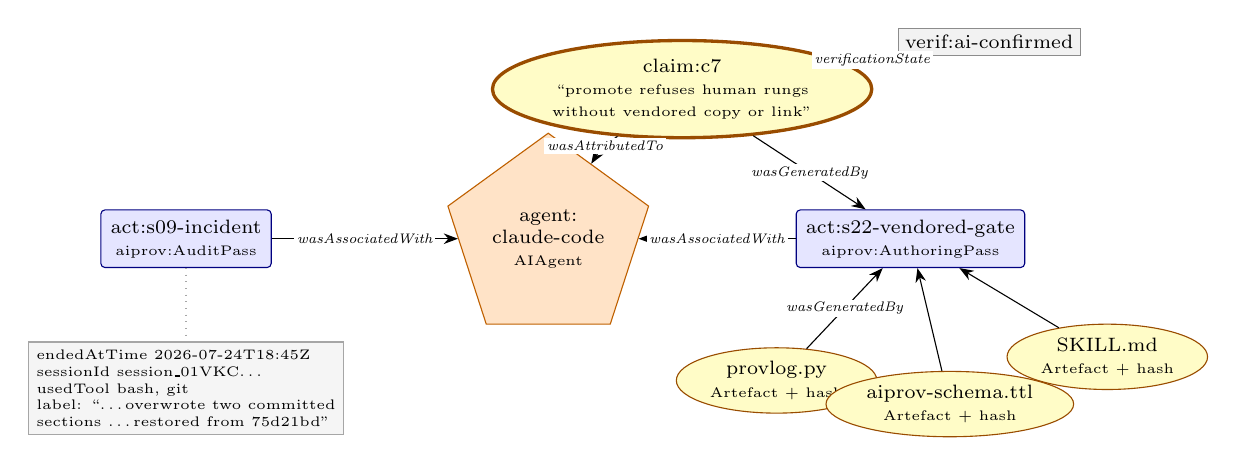
\begin{tikzpicture}[
  font=\scriptsize,
  act/.style={draw=blue!50!black, fill=blue!10, rounded corners=1.5pt,
              align=center, inner sep=3.5pt},
  ent/.style={draw=orange!60!black, fill=yellow!22, ellipse,
              align=center, inner sep=1.5pt},
  clm/.style={ent, very thick},
  ag/.style={draw=orange!75!black, fill=orange!22, regular polygon,
             regular polygon sides=5, inner sep=1.5pt, align=center},
  st/.style={draw=black!45, fill=black!5, align=center, inner sep=2.5pt},
  attr/.style={draw=black!35, fill=black!4, align=left, inner sep=3pt,
               font=\tiny},
  lbl/.style={font=\tiny\itshape, fill=white, inner sep=1pt},
  e/.style={-{Stealth[length=1.8mm]}}]
% shared agent
\node[ag] (agent) at (0,0) {agent:\\claude-code\\\tiny AIAgent};
% (a) mishap: s09-incident
\node[act] (s09) at (-4.6,0) {act:s09-incident\\\tiny aiprov:AuditPass};
\node[attr] (s09a) at (-4.6,-1.9) {endedAtTime 2026-07-24T18:45Z\\
sessionId session\_01VKC\ldots\\ usedTool bash, git\\
label: ``\ldots overwrote two committed\\
sections \ldots restored from 75d21bd''};
\draw[e] (s09) -- node[lbl]{wasAssociatedWith} (agent);
\draw[black!35, dotted] (s09) -- (s09a);
% (b) redesign: s22-vendored-gate
\node[act] (s22) at (4.6,0) {act:s22-vendored-gate\\\tiny aiprov:AuthoringPass};
\draw[e] (s22) -- node[lbl]{wasAssociatedWith} (agent);
\node[ent] (e1) at (2.9,-1.8) {provlog.py\\\tiny Artefact + hash};
\node[ent] (e2) at (5.1,-2.1) {aiprov-schema.ttl\\\tiny Artefact + hash};
\node[ent] (e3) at (7.1,-1.5) {SKILL.md\\\tiny Artefact + hash};
\draw[e] (e1) -- node[lbl]{wasGeneratedBy} (s22);
\draw[e] (e2) -- (s22);
\draw[e] (e3) -- (s22);
\node[clm] (c7) at (1.7,1.9) {claim:c7\\\tiny ``promote refuses human rungs\\\tiny without vendored copy or link''};
\node[st] (vs) at (5.6,2.5) {verif:ai-confirmed};
\draw[e] (c7) -- node[lbl]{wasGeneratedBy} (s22);
\draw[e] (c7) to[bend right=12] node[lbl, pos=0.4]{wasAttributedTo} (agent);
\draw[e] (c7) -- node[lbl]{verificationState} (vs);
\end{tikzpicture}
\caption{Two incidents from this experiment, exactly as the graph
represents them (node contents abridged from real triples). Left, a
mishap: the agent overwrote two committed manuscript sections; the
self-report is an \texttt{AuditPass} carrying timestamp, session,
tools, and the restoring commit in its label. Right, a contested
design: the operator challenged the \texttt{source-vendored} rung's
semantics; the redesign activity generated new tool and schema
versions (content-hashed artefacts), and its enforcement claim sits at
\texttt{ai-confirmed} after test-run. The incident vocabulary is just
the ordinary vocabulary.}
\label{fig:incident}
\end{figure*}

% 5.4 Division of labour as data — classify this experiment's recorded
%     activities by what triggered them: human contributions were
%     direction, lineage, people, and judgement calls; AI activities
%     were verification mechanics (registry resolution, hashing,
%     validation, builds). The graph makes the "AI absorbs tedium,
%     humans connect ideas and people" hypothesis (§6.9) empirically
%     inspectable rather than anecdotal — for this one experiment.
% 5.5 What the auditor can and cannot verify — hashes, commits, DOIs,
%     rung grants are checkable; honesty of self-reported telemetry is
%     not (bridge to §6).

\begin{table}[t]
\caption{Telemetry report of this paper's production (generated by
\texttt{provlog.py report} at submission; values from the provenance
graph, absent telemetry omitted).}
\label{tab:telemetry}
\centering
% TODO(build pass): generate via provlog.py report near submission.
\begin{tabular}{lr}
\toprule
Metric & Value \\
\midrule
Activities / claims / sources & --- \\
Tokens (input / output / cache) & --- \\
Cost & --- \\
Rung distribution & --- \\
\bottomrule
\end{tabular}
\end{table}

\begin{figure}[t]
\centering
% TODO(F4, build pass): provlog.py extract --seed-types Artefact Claim
% -> dashboard SVG export of the subgraph that contributed to main.pdf.
\fbox{\parbox[c][4.2cm][c]{0.9\linewidth}{\centering\itshape
F4 placeholder: provenance subgraph of this paper (generated)}}
\caption{Backward provenance closure of this paper: the activities,
agents, sources, and prompts that contributed to the PDF you are
reading.}
\label{fig:graph}
\end{figure}

\section{Discussion and Limitations}\label{sec:discussion}

\textbf{Self-report honesty.} The graph is only as truthful as its
writer. Mitigations are structural rather than rhetorical: content
hashes and commit bindings tie records to bytes, validation runs
server-side in CI, the omit-don't-estimate rule removes the temptation
of invented precision, and the human-only rungs cap what an AI may
assert about its own work. The overwrite incident of
Section~\ref{sec:meta} shows the mitigation working: with the
repository as the process substrate, an AI mistake was a recoverable,
recorded event rather than silent corruption.

\textbf{Why human-only rungs stay human.} \texttt{ai-confirmed} is a
machine judgement with known failure
modes~\cite{ai-hallucination2023}. The ladder does not pretend
otherwise; it makes the judgement's author explicit instead of
laundering machine confidence into apparent human endorsement.

\textbf{Cost, and a gap that half closed.} The method's overhead in
this experiment was one logging command and one extra commit per
working round, plus the audit activities the tooling writes itself.
Token telemetry illustrates the omit-don't-estimate rule in motion:
the harness exposes no live usage to the agent, so nothing was
recorded at first; when the operator challenged the gap, the session
record turned out to carry the provider's per-request usage blocks,
and the totals in Table~\ref{tab:telemetry} were backfilled from
them, reported rather than estimated. The remaining gap is cost: the
record is unpriced, and assuming prices would fabricate. Honest cost
accounting in AI-assisted work still needs the provider to report it.
A larger question stays open behind the numbers. This one session
consumed 185~million cache-read tokens to produce one draft paper and
one method release; whether that expenditure justifies its
environmental footprint and its other costs is a debate this paper
does not settle and does not want to hide. The schema reserves
\texttt{aiprov:energyWh} for exactly this reason, and it sits empty
here because no provider reported energy. Our position is only that
the debate should be held over recorded consumption rather than
guesses, in either direction: neither dismissing AI assistance as
obviously wasteful nor excusing it as obviously worthwhile. The graph
makes the bill legible; whether it is worth paying is a judgement the
record enables but cannot make.

\textbf{Skill drift.} The method evolved mid-experiment, v0 to v0.8,
including two operator-contested ladder redesigns. Immutable archived
snapshots, a changelog, and per-activity commit binding keep every
run attributable to the exact method version in force, so evolution
does not blur attribution.

\textbf{Practices that emerged.} Three are small enough to adopt
tomorrow. Registry-fetched citation metadata: every BibTeX entry comes
from doi.org content negotiation, never typed from memory, a concrete
discipline against fabricated
references~\cite{fabricated-citations2023}; the one failure was
infrastructural, a registry serving malformed BibTeX, and CI caught
it, not a reader. Registry-resolved identities: the operator,
acknowledged colleagues, and co-authors enter the record via ORCID
lookups, extending never-fabricate from telemetry to social metadata.
Verified-before-cited: no reference appears in the bibliography
without a ladder-backed source node, making the bibliography a view of
the graph rather than a hand-maintained list.

\textbf{Transparent self-citation.} No-parentless-claim forces citing
one's own priors; the lineage of Section~\ref{sec:background} is the
author's own repositories and specifications. Self-citation is
frowned upon as metric gaming, yet unavoidable as provenance. The
resolution is transparency instead of omission: sources carry
\texttt{aiprov:selfCitation}, the report prints the ratio (here 4 of
31), and a reviewer can judge necessity per source. The test that
separates influence from inflation: a transparent self-citation is
load-bearing, removing it would orphan a lineage or method claim, and
it points at repositories and specifications rather than
metric-bearing venues. It declares descent; it does not farm
citations.

\textbf{Regulatory alignment.} The EU AI Act's transparency rules ask
for disclosure and machine-readable marking of AI-generated
content~\cite{eu-ai-act2024}. A provenance graph is exactly that
marking, and because CI derives the disclosure statement from the
graph on every build, the published statement cannot lag the record.
Provenance-first authoring turns a compliance duty into a by-product.

\textbf{Generality.} Beyond papers, the same invariants and ladder
apply to code, data pipelines, CAD models, and AAS
submodels~\cite{aas-part1-v30rc02}; what remains domain work is the
choice of entity subclasses. The AAS case bridges to the outlook:
digital-twin ecosystems already assume machine-readable semantics, so
AI-work provenance slots in as one more submodel concern rather than a
foreign add-on.

\textbf{The force multiplier, both ways, and the optimistic reading.}
One operator ran method, paper, and integration fork in parallel
during this experiment; unaccounted, the same multiplication is the
dilution engine of Section~\ref{sec:dilution}. The differentiator is
not speed but auditability: fast work that carries its record is
distinguishable from fast noise. Fast paper, slow ideas is the honest
reading of this project, and only the graph makes that reading
checkable. There is also a hopeful version of the same observation.
What the multiplication buys is not mainly volume: AI absorbing the
tedium, registry lookups, hash binding, conformance checks, build
plumbing, can free human attention for the two things machines do not
supply, connecting ideas and connecting people. This experiment's own
activity log shows that division of labour. No guarantee, only a
chance; a provenance graph is how one would check, later, whether the
chance was taken.

\section{Conclusion}\label{sec:conclusion}

We generalized the F(AI)\textsuperscript{2}R method into aiprov, a
domain-agnostic PROV-O extension for AI-in-the-loop work; we packaged
the method as an executable skill an AI agent operates itself; and we
applied it to its own production, mishaps, mid-experiment redesigns,
and all. The stance of the original experiment carries over and
extends: the repository is the paper, is the process, and now also is
the method, versioned, validated, and shipped alongside what it
produced.

Three roots converge here: AI-assisted research practice, which
contributed transcript-as-artifact; engineering provenance, which
insists on traceability; and industrial semantic modeling, which
taught that where exchange matters, semantics must be formal. Where
semantics are important, provenance is the semantics of work.

The path forward is infrastructure. shepard~\cite{shepard}, a jointly
developed DLR system for heterogeneous product and research data,
already serves as the data backbone of engineering deployments such as
the MEMAS additive-manufacturing pipeline~\cite{memas2024}; an
experimental fork~\cite{shepard-fork} is the staging ground for
integrating aiprov into it as planned work. Where shepard instances
capture what was produced and measured, aiprov adds who, human or AI,
shaped it and how it was verified. Further work includes multi-agent
attribution, energy accounting, registry integration beyond ORCID and
DOI, vendoring sources at the access gate by default, and a combined
profile with uncertainty-aware provenance~\cite{uncertainty-prov2026}.


\section*{Acknowledgment and AI Transparency Statement}
The ideas in this paper were sharpened through earlier
experiments~\cite{obscurity-is-dead, fair2r-repo}; through discussions
in the context of the Helmholtz Metadata Collaboration
(HMC)~\cite{hmc}: with Witold Arndt in the HMC hub for
aeronautics, space and transport, and through the broad view of AI in
research afforded by chairing the HMC Conference 2025 programme
committee~\cite{hmc-conference2025}; through exchanges with Frank
Dressel on provenance for engineering
systems~\cite{uncertainty-prov2026}; through deep discussions with
Sirko Schindler and Carsten Hoyer-Klick on ontologies; through the
research-data-management evangelism of Christian Langenbach at DLR;
and through the inspiration of Carina Haupt's work on provenance
use cases~\cite{provenance-overview2022} and of the MEMAS project's
integrated data management~\cite{memas2024}.

This paper and its repository were produced with an AI agent operating
the ai-provenance skill; every activity, generated artefact, claim, and
source is recorded in the version-controlled provenance graph,
including the production of this statement. The following disclosure is
generated from that graph by \texttt{provlog.py disclosure} and is made
in view of the transparency rules of the EU Artificial Intelligence
Act~\cite{eu-ai-act2024}:

\begingroup\itshape
% Generated by provlog.py disclosure — do not edit by hand.
Parts of this work were generated or edited with the assistance of artificial-intelligence systems: Claude Code (Claude Fable 5, Anthropic), associated with 23 recorded activities. In line with the transparency obligations for AI-generated content under Regulation (EU) 2024/1689 (AI Act), this assistance is disclosed here and is additionally marked in machine-readable form: the version-controlled provenance graph (provenance.ttl, W3C PROV-O) records the 23 activities behind this work, the 23 generated artefacts with content hashes, and the 5 recorded claims with their verification states. Human oversight is structural: verification rungs above ai-confirmed are reserved to human agents, and the conformance validator rejects AI-granted promotions.

\endgroup

\emph{Availability:} skill bundle, provenance graph, transcripts,
and paper sources are public at
\url{https://github.com/noheton/f-ai2-r}; the skill loads in any
Agent Skills client, and conformance-gated releases carry bundle,
PDF, graph, and checksums. A preprint of this article is available
on arXiv.

\emph{Competing interests:} the author declares none.

\emph{Funding:} no dedicated funding; author employed by DLR.

\bibliographystyle{IEEEtran}
\bibliography{../paper/references}

\end{document}
